\documentclass[10pt,preprint]{aastex}
\usepackage{amsmath}
\usepackage{breqn}
\usepackage{cite,natbib}
\usepackage{epsfig}
\usepackage{cases}
\usepackage[section]{placeins}
\usepackage{graphicx, subfigure}
\usepackage{color}
\usepackage{amsmath}
\usepackage{float}
\floatplacement{figure}{H}
% \usepackage[nomarkers,figuresonly]{endfloat}

\newcommand{\logg}{log \emph{g}~}
\newcommand{\teff}{$T_{eff}~$}
\newcommand{\prot}{$P_{rot}~$}

\newcommand{\ah}{$\hat{A}_n$}
\newcommand{\ph}{$\hat{P}_n$}
\newcommand{\ch}{$\hat{C}_n$}
\newcommand{\gh}{$\hat{G}_n$}
\newcommand{\yh}{$\hat{Y}_n$}
\newcommand{\teffh}{$\hat{T}_n$}

\newcommand{\feh}{[Fe/H]}
\newcommand{\dd}{\ensuremath{\,\mathrm{d}}}

\begin{document}

\title{Calibrating Gyrochronology using Kepler Asteroseismic targets}

\author{Ruth Angus$^1$, Suzanne Aigrain$^1$, Amy McQuillan$^2$, Daniel Foreman-Mackey$^3$,  William, J. Chaplin$^4$, Tsevi Mazeh$^2$}
\affil{$^1$Department of Physics, University of Oxford, OX1 3RH, UK}
\affil{$^2$School of Physics and Astronomy, Raymond and Beverly Sackler, Faculty of Exact Sciences, Tel Aviv University, 69978, Tel Aviv, Israel}
\affil{$^3$Centre for Cosmology and Particle Physics, New York University, New York, NY, USA}
\affil{$^4$School of Physics and Astronomy, University of Birmingham, Edgbaston, Birmingham, B15 2TT, UK}

\begin{abstract}
\label{abs}

Measuring ages for intermediate and low-mass stars on the main
sequence is challenging, but important for a wide range of studies,
from Galactic dynamics to stellar and planetary evolution.
Among the available methods, gyrochronology is a powerful one, because it requires knowledge of only the star�s mass (or colour) and its rotation period.
However, it is not well calibrated at late ages, and suffers from large uncertainties.
Asteroseismology provides relatively precise age measurements for some of the brightest stars observed by Kepler.
We measured the photometric rotation periods of 153 stars with asteroseismic ages in order to calibrate the gyrochronology relation and improve upon current methods of measuring the ages of MS field stars.
We use advanced statistical methods to model the relationship between rotation period, age, and mass (or colour or effective temperature) while accounting for measurement uncertainties in all three quantities.
Our sample includes both main sequence stars and subgiants, and straddles the Kraft break (only main sequence stars cooler than the Kraft break, $\sim$ 6250 K, are expected to follow gyrochronology relations); and this must be taken into account when modelling the data.
Our method has been applied to the extended sample of published rotation periods for stars with reliable mass and age estimates, and enables us to estimate ages for any star with a measured period and mass (or temperature), along with associated uncertainties that reflect both measurement errors and the intrinsic scatter in the gyrochronology relations.

\end{abstract}

\section{Introduction}
\label{intro}

Stellar ages are notoriously difficult to measure for main sequence (MS) stars; uncertainties are typically above the 20\% level \citep{Soderblom2010}.
% Chromospheric activity is often used as an age indicator, as well as lithium depletion, but the evolution of these properties on the main-sequence is poorly understood, plus, high resolution spectra are required to measure either of these properties.
Fitting isochrones to spectroscopic properties is one of the most commonly used dating methods for field stars, however this process is model-dependent, imprecise and requires high resolution spectroscopy.
Ages of field stars measured via isochrone placement often have uncertainties of order 100\% or more.
Gyrochronology has become a popular dating method due to its simplicity---knowledge of a star's rotation period and mass, or appropriate proxy, are the only requirements.
Thanks to the high-precision photometry delivered by the Kepler spacecraft, photometric rotation periods are now relatively easy to measure.

Cluster ages measured by fitting isochrones to an ensemble of coeval stars can have uncertainties as low as 10\%.
Open clusters are therefore invaluable tools for calibrating model dependent, empirical dating methods such as gyrochronology.
Unfortunately the majority of nearby clusters are young---there is a significant dearth of precisely measured ages for old stars and it is for this reason that the current gyrochronology relations are poorly calibrated at late ages.
The older Kepler clusters will provide excellent anchors for gyrochronology.
The Kepler cluster study \citep{Meibom2011} aims to measure rotation periods for stars in all four open clusters in the Kepler field of view: NGC 6866 (0.5 Gyr), NGC 6811 (1.1 Gyr), NGC 6819 (2.5 Gyr) and NGC 6791 (9 Gyr).
So far, rotation periods for 71 stars in NGC 6811 have been measured and member identification for the other three clusters is underway.
The gyrochronology relation of \citet{Barnes2007} relates stellar rotation period to age and B-V colour.
It was calibrated with 9 young open clusters, aged 650 Myrs or less, and the Sun; the clusters provided the period-mass dependence and the Sun provided the period-age dependence.
This gyrochronology relation was updated by \citet{Mamajek2008} who used activity indicators in young cluster stars and a small number of field stars.
% Chromospheric activity, usually measured from the strength of emission in the centers of the broad Ca II H \& K emission lines $R'_{HK}$, is driven by the magnetic dynamo and therefore correlated with rotation (\citet{Kraft1967}, \citet{Noyes1984}, \citet{Montesinos2001}).
The evolution of stellar activity is still poorly understood, especially for older stars and whilst the \citet{Mamajek2008} relation improves upon the period-colour dependence of the \citet{Barnes2007} relation, it still relies almost exclusively on the Sun for its age dependence.

\subsection{Angular momentum loss in Main Sequence stars}

Stellar winds are constrained to corotate with the stellar surface out to the Alfv\`{e}n radius \citep{Weber1967}, at which point the stellar wind decouples and angular momentum is lost from the star.
% Stars lose angular momentum over their MS lifetimes via a magnetised wind that is constrained to rotate with the stellar surface out to the Alfv\`{e}n radius \citep{Weber_1967}.
The strength of the magnetic field at the stellar surface, and therefore the rate of angular momentum loss, is inversely proportional to rotation period \citep{Kawaler1988}.
So although stellar populations are born with a range of rotation periods, the rapid rotators rapidly lose angular momentum and rotation periods converge onto a unique sequence.
The timescale for convergence is around the age of the Hyades: 650 Myrs \citep{Irwin2009}, after this time rotation periods are \emph{independent} of their initial values.
The rate of angular momentum loss also depends on stellar mass---more massive stars lose angular momentum more slowly and in theory stellar age can be inferred from mass (or some proxy thereof) and rotation period measurements alone.
% Due to this dependence all F, G and K stars converge onto a unique mass-period-age relation at around the age of the Hyades: 650 Myrs \citep{Irwin_2009}.
The gyrochronology relation of \citet{Barnes2007} can be written:

\begin{equation}
P = A^n \times a(B-V-c)^b
\label{eq:Barnes2007_2}
\end{equation}

where P, A,  B and V are rotation period (in days), age (in Myr),  and B and V band colours respectively. The values of n, a, b and c are tabulated in \ref{tab:constants}.
This relation was further calibrated by \citep{Mamajek2008}, using chromospheric activity measurements of field stars. %citation needed
Their relation takes the same form as Barnes (2007) with revised parameters shown in table \ref{tab:constants}.
Note that \citet{Mamajek2008} treat c, the parameter setting the position of the colour discontinuity, as a free parameter, whereas \citet{Barnes2007} fix it at 0.4.
% As a result, the \citet{Barnes2007} relation can be applied to hotter stars.

\begin{deluxetable}{lcc}
\label{tab:constants}
\tablewidth{0pc}
\tablecaption{Values of a, b, c \& n in \citet{Barnes2007} and \citet{Mamajek2008}}
\tablehead{
\colhead{Parameter}&
	\colhead{\citet{Barnes2007}}&
\colhead{\citet{Mamajek2008}}}
\startdata
a & $0.7725 \pm 0.011$ & $0.407 \pm 0.021$ \\
b & $0.601 \pm 0.024$ & $0.325 \pm 0.024$ \\
c & $0.4$ & $0.495 \pm 0.010$ \\
n & $0.5189 \pm 0.0070$ & $0.566 \pm 0.008$ \\
\enddata
\end{deluxetable}

Gyrochronology relations of this kind can only be applied to F, G and K MS stars.
M dwarfs are fully convective and have a different magnetic dynamo \citep{McQuillan2013}, therefore follow a different spin-down law.
% Which is What?
% However, M dwarfs are unsuitable targets for asteroseismology as they do not display high signal-to-noise Solar-like oscillations and so do not feature in our sample anyway.
Stars with effective temperatures $\gtrsim$ 6250 K have shallow convective zones - they are almost fully radiative - and, again, they have a different dynamo-driven magnetic field \citep{Kraft1967}.
These massive stars retain their initial rotation period throughout their brief MS lifetimes and are therefore not suitable gyrochronology targets.

This paper is laid out as follows: the asteroseismic data are described in \textsection~\ref{sec:asteroseismic_targets}, our rotation period measurement method is described in \textsection~\ref{sec:rotation_period_measurement}, the calibration and model fitting process is outlined in \textsection~\ref{sec:gyro_cal} and the results are discussed in \textsection~\ref{sec:results}.

\section{Asteroseismic ages}
\label{sec:asteroseismic_targets}

% Ages measured with asteroseismology can be very precise, with uncertainties as low as 10\% in some cases (\citet{Brown1994}, \citet{SilvaAguirre2013}).
% Unlike rotation based age diagnostics, the precision of asteroseismic ages are not themselves age dependent.
% Rotation periods increase with age and longer rotation periods are more difficult to measure, therefore the precision of rotationally derived stellar ages is also age dependent.
% The signal-to-noise ratio of asteroseismic oscillations remains relatively stable throughout a star's MS lifetime and therefore the precision of asteroseismic ages is age independent. {\color{red}(CITATION)}.
Acoustic (pressure) mode oscillations produce periodic luminosity variations on timescales of $\sim$ 5 minutes in Solar-like stars.
These oscillations can be detected in short-cadence Kepler data---a fourier transform of the time series reveals a series of narrow peaks at discrete frequencies, overtones of high radial order, n.
Non-radial oscillations with angular degree, l are also detectable in Solar-like stars.
The frequency spacing, (or large frequency separation, $\Delta\nu_{nl} = \nu_{n+1l}-\nu_{nl}$) between consecutive overtones, n, of the same degree, l, is a fundamental asteroseismic observable.
% The mean large frequency separation between oscillation modes, $\Delta\nu$, is a fundamental asteroseismic observable and is related to stellar density.
% $\Delta\nu \propto \sqrt\rho_{star}$
The series of peaks in the Fourier transform is modulated by a gaussian envelope, the maximum of which is another fundamental asteroseismic observable, $\nu_{max}$.
% When combined with spectroscopic observations and compared with theoretical stellar evolution models, measurements of the two fundamental asteroseismic observables yeild stellar ages.
These two fundamental asteroseismic parameters together with effective temperature can be used, via the scaling relations below, to derive stellar masses and radii.

\begin{equation}
\frac{\Delta\nu}{\Delta\nu_{\odot}} \approx \sqrt{\frac{M/M_{\odot}}{R/R_{\odot}^3}}
\label{eq:delta_nu}
\end{equation}

\begin{equation}
\frac{\nu_{max}}{\nu_{max,\odot}} \approx \frac{M/M_{\odot}}{(R/R_{\odot})^2\sqrt{(T_{eff}/T_{eff,\odot})}}
\label{eq:delta_nu}
\end{equation}

In particular, the mean large frequency separation, $\Delta\nu$ is proportional to the mean stellar density.

\citet{Chaplin2013} Calculated the ages of 505 Kepler targets using the above scaling relations with estimates of $\Delta\nu$ and $\nu_{max}$.
A grid-based approach was used to measure stellar properties: values of $\Delta\nu$ were calculated for each R and M on the grid and compared with the observed $\Delta\nu$.
Ages quoted in \citet{Chaplin2013} are the combined result of six different grid-based model pipelines.
The uncertainties on the ages reflect the model dependencies.
Two sets of effective temperatures were used: one was derived using an Infra-Red Flux Method (IRFM) calibration (\citet{Casagrande2010}, \citet{SilvaAguirre2012}) and the other from a recalibration of the SDSS griz filter KIC photometry by \citet{Pinsonneault2012} using Yale Rotating Stellar Evolution Code (YREC) models \citep{Demarque2004}.
We use the second set of temperatures since they are slightly more precise.
% test: is our analysis sensitive to this choice?

The asteroseismic ages in \citet{Chaplin2013} have typical uncertainties of $\sim$ 35\%; however, it will be possible to derive more precise ages for some of these stars.
By measuring the frequency of each oscillation mode individually, not just the mean large serparation, one can build up a density profile of the star and provide a tighter constraint on its age.
Ages derived from individual oscillation mode measurements can have uncertainties as small as 10\% (\citet{Brown1994}, \citet{SilvaAguirre2013}, however measuring frequencies for individual oscillation modes is a manual process and can only be applied in the highest signal-to-noise cases.
\citet{Chaplin2013} predict that around 150 of the 505 stars will be suitable for this individual oscillation mode treatment.
% Although asteroseismology is a potentially precise dating method, it can only be applied to bright stars observed by missions like Kepler that show solar-like oscillations \citep{Chaplin_2011}.
% It is therefore essential that we have a well calibrated dating method like gyrochronology which can be applied to any F, G or K star with a measurable rotation period.
So far this has been done for 65 of the 505 with the Asteroseismic Modeling Portal (AMP), 42 of which are published in \citep{Metcalfe2014} and 23 obtained from Silva Aguirre (private communication).
Of the 42 stars in \citep{Metcalfe2014}, we only integrate the `simple stars' (cool dwarfs) into our sample---we ignore the `F stars' and `mixed mode' (subgiant) stars as these are not expected to follow the simple gyrochronology relation.
% {\color{red} Shouldn't I include these to be consistent?}
The AMP uses the `peak bagging' technique \citep{Appourchaux2012} to measure individual oscillation mode frequencies.
% (typically improved by a factor of $\sim$ 2), by measuring the frequency of individual oscillation modes, using the `peak bagging' technique \citep{Appourchaux2012}.
Precise effective temperatures and metallicities were obtained from \citet{Bruntt2012}.
% The uncertainties of stellar ages measured with AMP are typically improved over the scaling relation techique by a factor of 2.

% Infra-Red Flux Method (IRFM) calibration (Casagrande et al. 2010; see also Silva Aguirre et al. 2012). This made use of multi-band JHK photometry from the Two Micron All Sky Survey (2MASS; Skrutskie et al. 2006), photometry in the SDSS griz bands available in the KIC, and reddening estimates from Drimmel et al. (2003). A second set of temperatures were those derived by Pinsonneault et al. (2012), who performed a recalibration of the KIC photometry in the SDSS griz filters, using YREC models. The complementary photometry that was available to us did not allow strong constraints to be placed on the metallicity of all the targets. When using the photometric Te� in the grid searches we therefore adopted an [Fe/H] corresponding to an average value for the field of 0.2�0.3 dex (e.g. see Silva Aguirre et al. 2011).

% SHOW 3D FIGURE

\section{Rotation Period Measurements}
\label{rotation_period_measurement}

The Kepler light curves of these 505 asteroseismic targets display quasi-periodic variations on timescales corresponding to rotational periods of the stars.
Flux variations are produced by active regions on the stellar surface, rotating in and out of view.
In order to measure periodic signals in the light curves we used the auto-correlation function (ACF) method, developed by \citet{McQuillan2013}.
An autocorrelation function describes the self-similarity of a light curve at a range of lags and the highest peak in the ACF (usually also the first peak) is centered on the dominant periodic signal in the time series.
As an alternative to the standard Fourier decomposition and least-squares fitting of sinusoidal models \citep{Zechmeister}, autocorrelation is better suited to signals that are not sinusoidal or strictly periodic and is more effective at distinguishing a true signal from its harmonics and sub-harmonics.
For a more detailed description of the advantages of the ACF method over sine-fitting periodograms, see \citet{McQuillan}.

Long cadence PDC-MAP data were used throughout this analysis (\citet{Smith_2012}, \citet{Stumpe_2012}).
The PDC-MAP data are the product of an initial systematics removal process applied by the Kepler team, in which large-scale linear trends are removed in order to improve planet transit search and modelling capability.
PDC-MAP data are not, however, optimised to preserve stellar variability: periodic signals longer than around 30 days are reduced in power.
Additionally, light curves still contain large systematic features, such as the exponential decays that appear after telescope shutdowns, which affect period measurement precision.
The Astrophysically Robust Correction (ARC) is a detrending method developed by \citet{Roberts2013} is better at preserving astrophysical signals, however, it has not yet been applied to all Kepler quarters, so we opt to use PDC-MAP.
% {\color{red} So why are we still using it then?! - explain!}
% Note - I HAVE done some injection tests... could talk about these, although it would probably involve quite a lot more work...

In our implementation of the ACF method the first two peaks in the ACF were identified and the central value of the first peak was temporarily accepted as the period (unless the second peak was higher than the first in which case {\it its} central value was taken).

Note that an important advantage of the ACF method over a periodogram approach is in its ability to differentiate between harmonic signals produced by multiple active regions on the stellar surface from the true periodic signal: these scenarios usually produce ACFs in which the second peak is higher than the first.
Subsequent peaks in the ACF lying within 10\% of an integer multiple of the period were identified.
The final, reported period is calculated from the mean separation between peaks that lie at integer multiples of the period and the uncertainty on the period is calculated from the distribution of central peak values.
Measuring the mean peak separation removes a bias that can sometimes be introduced when a long-term, slowly decaying trend dominates the ACF at small periods.
If the first ACF peak is small when superimposed onto this trend, the period will be underestimated as the central peak value will be shifted towards smaller periods.
In cases where only one peak was present in the ACF, i.e. for stars with periods that are a significant fraction of the time coverage of a Kepler quarter, the central peak value was kept as the period and the uncertainty measured from the width of the peak.
Example ACFs for Kepler light curves are shown in figure \ref{fig:subfigures} at the end of this document.
An example light curve and ACF for KIC 322300 is shown in figure \ref{fig:lc} and quarter-by-quarter period measurements in figure \ref{fig:ind_qs}.
All but one of the quarters for this star produced an ACF with a significant initial peak and repeating subsequent peaks and, of those, all period measurements lie within 15\% of the median value.

We used Kepler quarters 3-16 to measure rotation periods for the stars in our sample.
While some light curves displayed high amplitude, regular flux variations produced by star spots, others were dominated by random noise or instrumental systematics.
To ensure that the periodicities measured were truly representative of stellar rotation periods, we computed an ACF for each Kepler quarter, individually, for each star and required that the resulting periods were mutually consistent.
We required that period measurements lie within 15\% of the median period value, or within 15\% of twice and half the median in order to catch aliases.
The maximum period, detectable in one Kepler quarter with our ACF method was just over 20 days.
% Why? 90 / 2 = 45, /2 ~ 20
In order to include stars with rotation periods longer than 20 days, we also calculated ACFs for quarters 3-6, 7-11 and 12-15, joined together.
Those stars with rotation periods consitent across all three years were examined by eye and included in our sample if a reasonable rotation period was measured.
The final, reported rotation periods were calculated from quarters 3-16, joined together.

Of the 505 targets in the original sample 122 rotation periods were reliably measured using the above process.
We added an additional 31 targets with rotation periods measured by \citet{McQuillan_2014}, increasing our sample to 153.
Of those 153, 13 of them have precise asteroseismic ages from AMP modelling.

\begin{figure}[ht]
\begin{center}
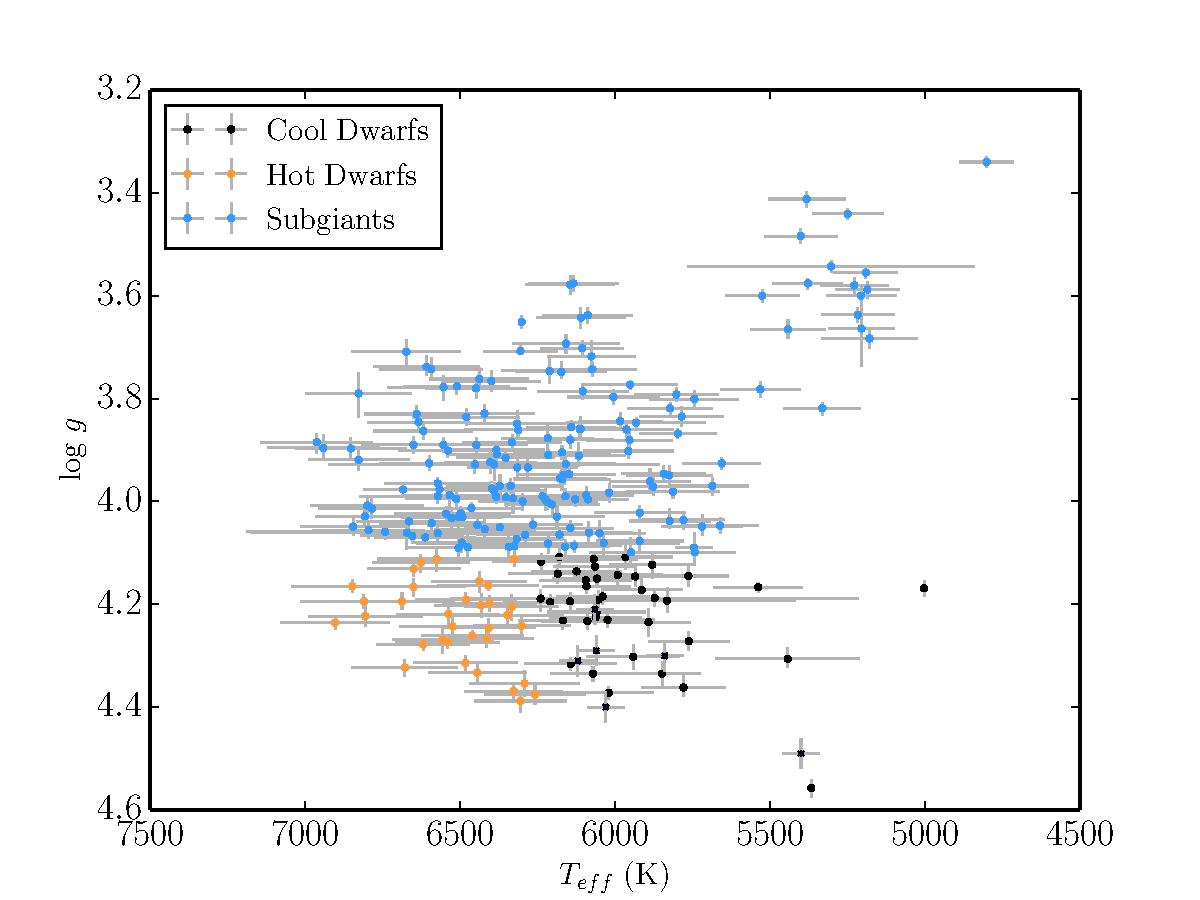
\includegraphics[width=6in, clip=true, trim=0 0 0.5in 0]{/Users/angusr/Python/Gyro/plots/logg_vs_t_paper.png}
\caption{\logg vs \teff for the 153 asteroseismic stars. Stars with \teff $>$ 6250 K are red and those with \logg $<$ 4.0 are blue. The triangular data points are those with precise ages. {\color{red}To do: add ASTEC isochrones}}
\label{fig:p_vs_a}
\end{center}
\end{figure}

\subsection{Supplementary data}

% 13 stars in our sample have  precise asteroseismic ages.
% 7 of these are from \citet{Metcalfe2012} with spectroscopic effective temperatures, metallicities and log g from \citet{Bruntt2012} and 6 are from Silva-Aguirre (private communication).
% The individual mode frequencies were measured for these stars, enabling a more detailed modelling of their interior structure and therefore yeilding a more precise age measurement.
% An unfortunate disharmony exists between asteroseismology and gyrochronology.
% Stellar rotation periods are easiest to measure for active, rapidly rotating stars, however these do not always make good asteroseismic targets.

The asteroseismic sample covers a large range of ages (see figure \ref{fig:p_vs_a}), however they do not provide good mass coverage at all ages.
There are very few stars with temperatures below 6000 K (B-V $\sim$ 0.55) and of the low mass stars, most of them are old.
We therefore added 260 young cluster stars to our sample from NGC6811, the Hyades and Praesepe.
{\color{red} Still need to add M37, Coma Ber, M11, M34, M35, M50, Pleiades, IC 2391, IC 2602}

\begin{figure}[ht]
\begin{center}
	\subfigure[$P_{rot}$ vs \teff]{
            \label{fig:p_vs_t}
	    \includegraphics[width=3in, clip=true, trim=0 0 0.5in 0]{/Users/angusr/Python/Gyro/plots/p_vs_t_paper.png}
        }
	\subfigure[$P_{rot}$ vs B-V colour]{
            \label{fig:p_vs_bv}
	    \includegraphics[width=3in, clip=true, trim=0 0 0.5in 0]{/Users/angusr/Python/Gyro/plots/p_vs_bv_paper.png}
        }
    \end{center}
    \caption{ Photometric rotation period vs effective temperature and B-V colour for 153 Kepler asteroseismic targets. \teff was converted to B-V using \citet{Sekigchi2000}.
     }
   \label{fig:subfigures}
\end{figure}

Rotation periods and B-V colours for the Hyades were obtained from \citet{Radick1987} and an age of 650 Myrs was adopted from \citet{Perryman1998}.
NGC 6811 is a cluster in the Kepler field with an age of 1.1 $\pm$ 0.2 Gyr \citep{Janes2011} with photometric rotation periods for cluster members measured by \citet{Meibom2011}.
These stars have g-r colours which were converted to dereddened B-V with $E_{(B-V)} = 0.1$.
Rotation periods for the 590 Myr \citep{Khalaj2013} cluster Praesepe were published in \citet{Kovacs2014}, with B and V colours from the APASS database ((http://www.aavso.org/apass).

A further 5 field stars with precise age measurements were added to the sample: 16 Cyg B, Alpha Cen A and B, 18 Sco and, of course, the Sun.
An asteroseismic age for 16 Cyg B was obtained from \citet{Metcalfe2012}, $T_{eff}$ from \citet{Ramirez2009} and rotation period from \citet{Henry2000} with B and V colours from \citet{Moffett1979}.
An age of 6 $\pm$ 1 Gyr was adopted for Alpha Cen AB, based on the analysis by \citet{Bazot2012} and \citet{Yildiz2007} (note that ages derived for Alpha Cen AB are extremely model dependent).
B and V colours were obtained from \citet{Mermilliod1986} and rotation periods from \citet{Hallam1991} and \citet{Dumusque2012} for A and B, respectively.
An age of 4.568 $\pm$ 0.001 Gyr for the Sun was taken from \citet{Bouvier2010}, and a rotation period from \citet{Donahue1996}, with same interpretation as in \citet{Mamajek2008}.
The age of 3.66 $\pm$ 0.2 for 18 Sco was taken from \citet{Li2012}, with rotation period from \citet{Petit2008} and B and V colours from \citet{Mermilliod1986}.

Despite having effective temperatures for the asteroseismic targets, we converted $T_{eff}$ to B-V colours, using the relation in \citet{Sekiguchi2000}---see figure \ref{fig:subfigures}.
This conversion is imprecise since the metallicites of the asteroseismic targets are the field average and not calculated per star, however we concluded that converting $T_{eff}$ to colour would be more efficient than converting cluster star colours to $T_{eff}$, since we have more information about the asteroseismic sample.

The entire set of 418 stars is shown in figure \ref{fig:3d}. Asteroseismic targets are shown in black, with supplementary cluster and field stars in red.

\begin{figure}[ht]
\begin{center}
\includegraphics[width=6in, clip=true, trim=0 0 0.5in 0]{/Users/angusr/Python/Gyro/plots/3d_angled.png}
\caption{Colour, age and rotation periods of all 418 stars. Asteroseismic stars are black and additional cluster and field stars are red. {\color{red}add precise stars.}}
\label{fig:3d}
\end{center}
\end{figure}
%
\begin{figure}[ht]
\begin{center}
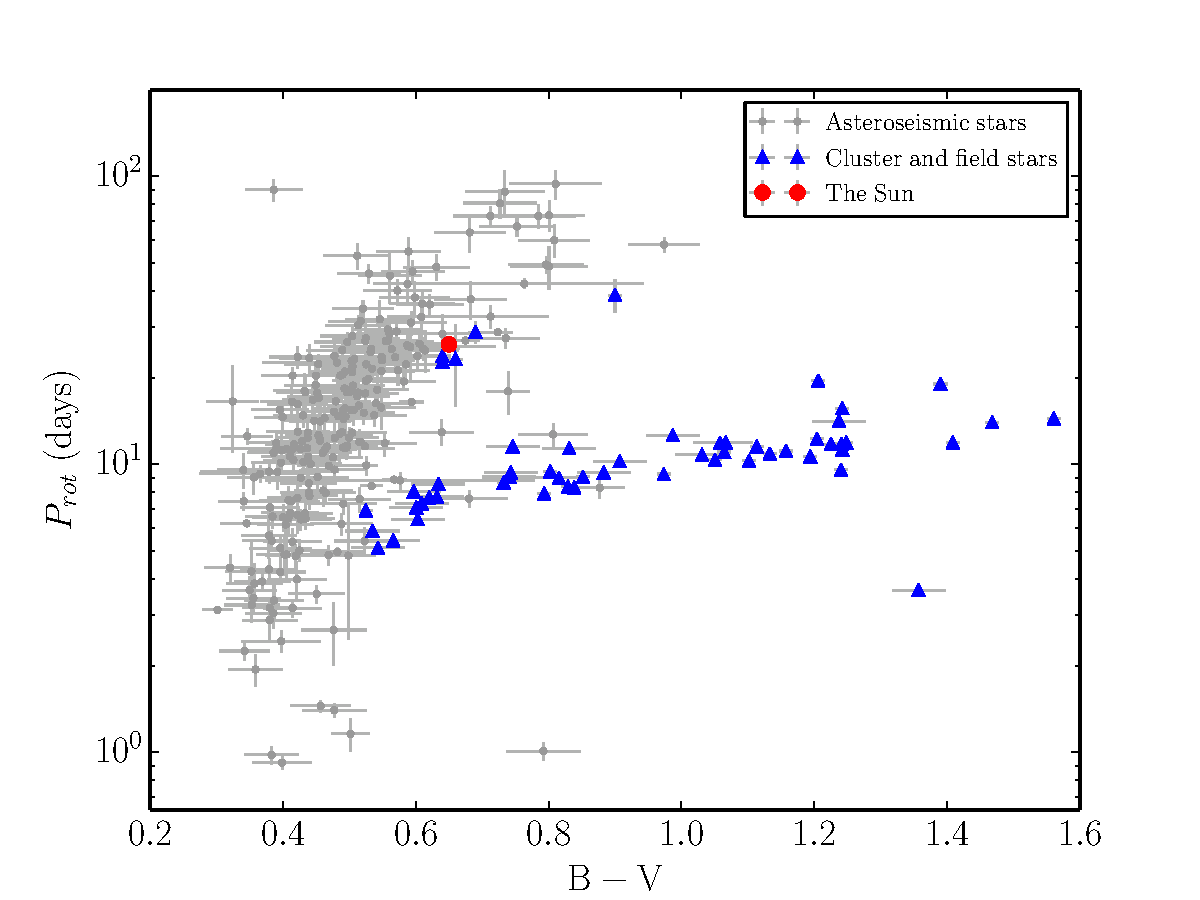
\includegraphics[width=6in, clip=true, trim=0 0 0.5in 0]{/Users/angusr/Python/Gyro/plots/p_vs_bv_paper2.png}
\caption{Photometric rotation period vs B-V colour for 153 Kepler targets (black) plus cluster and field stars (red). The blue stars have precise ages.}
\label{fig:3d}
\end{center}
\end{figure}
%
\begin{figure}[ht]
\begin{center}
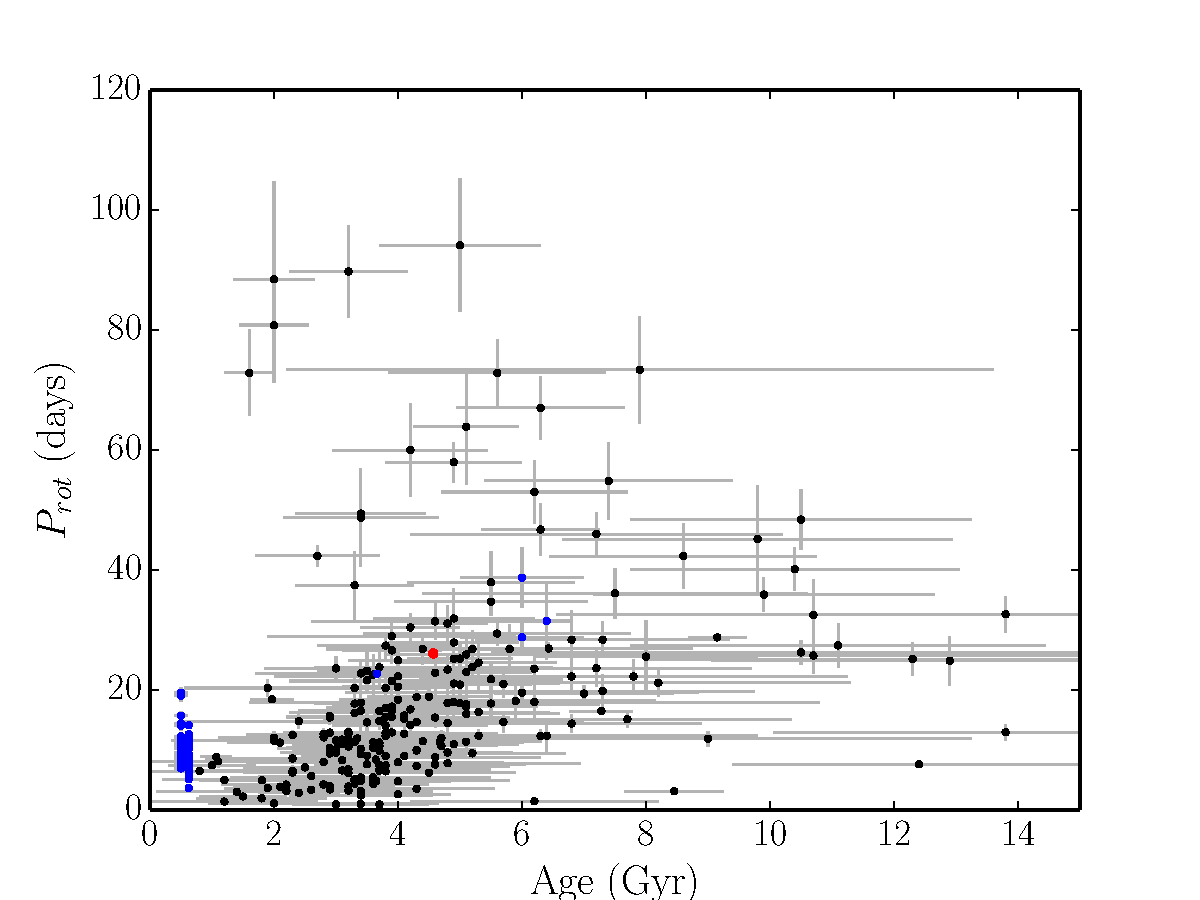
\includegraphics[width=6in, clip=true, trim=0 0 0.5in 0]{/Users/angusr/Python/Gyro/plots/p_vs_a_paper2.png}
\caption{Photometric rotation period vs age for 153 Kepler targets (black) plus cluster and field stars (red). The blue stars have precise ages. {\color{red} add 7 other precise stars.}}
\label{fig:p_vs_a}
\end{center}
\end{figure}

\section{Calibrating the Gyrochronology relation}
\label{sec:gyro_cal}

\subsection{The model}

The 153 asteroseismic stars in our sample have B-V colours converted from effective temperatures, photometric rotation periods, P and asteroseismically derived ages, A and surface gravities, \logg (G).
Each of these properties has an associated uncertainty, assumed to be independent and Gaussian for B-V and P and log-normal for A and G.
The 265 cluster and field stars added to our sample do not have \logg values; however, since we only use \logg to separate the populations of subgiants and dwarfs (and we assume that the cluster and field stars are dwarfs) this shouldn't hurt our analysis.

Gyrochronology is not applicable to hot stars or subgiants.
Stars with effective temperatures above the Kraft-break, $T_{eff} \sim$ 6250 K, \citep{Kraft1967} do not have a thick convective envelope and cannot support a strong magnetic dynamo, so do not spin down during their MS lifetimes.
Subgiants spin down rapidly as they expand due to angular momentum conservation and thus diverge from the gyrochronological mass-period-age plane.
The point in their evolution at which they turn off the `gyrochronological MS turnoff' is difficult to define.
% Although the point at which a star turns off the MS is relatively well known and understood, (conventionally its hottest point on the HR diagram), the point at which stars stop following the gyrochronology spin-down relation is less well understood.
Classically, MS turnoff is defined as the hottest point on a star's path on the HR diagram but theory predicts that evolving stars begin the process of spinning down relatively slowly after leaving the `classically defined' MS \citep{vanSaders2013}.
For this reason we choose a very simple definition of MS turnoff---we use a \logg cut of 4.0 to differentiate dwarfs from giants.

We do not simply exclude hot stars and subgiants from our sample during the modelling process---we model all three populations simultaneously.
This allows for the fact that stars have some probability mass lying in all three regimes due to their large observational uncertainties.

The gyrochronology relations of \citet{Barnes2007} and \citet{Mamajek2008} take the form:

\begin{equation}
P = A^n \times a(B-V-c)^b,
\end{equation}

where n, a, b and c are constants with values tabulated in \ref{tab:constants}.
Our relation will be of the form:

% \begin{equation}
% 	A = \left[\frac{P}{a(B-V - c)^{b}}\right]^{\frac{1}{n}}
% \label{eq:functional_form2}
% \end{equation}

\begin{equation}
A = \left[P \times \frac{1}{a}(B-V - c)^{-b}\right]^{\frac{1}{n}}
\label{eq:plane}
\end{equation}

Where, since we want to produce a predictive distribution for the age of a star given estimates of B-V and P, A is now the dependent variable.

In addition to hot stars and subgiants, there is further population of contaminating stars in our sample: rapid rotators.
Around 20 stars with rotation periods of less than $\sim$ 5 days do not lie on the standard gyrochronology mass-period-age plane.
These stars could plausibly be synchronised binaries or stars with unseen, close-in, massive planets (\citet{Poppenhaeger2014}, \citet{Beky2014})

We model four stellar populations simultaneously: cool MS stars, hot MS stars, subgiants and rapid rotators.
The hot MS stars are defined as those with B-V $<$ 0.45, corresponding to \teff $\approx$ 6250 K for Solar metallicity and \logg.
Since there is no dependence of age on rotation period for massive MS stars, their ages are modelled as a log-normal distribution with mean and variance, Y and V, free parameters.
Subgiant ages \emph{do} depend on period and $T_{eff}$; however, since we are not interested in the rotational properties of these stars for the purposes of gyrochronology calibration, we also model them with a log-normal distribution with mean and variance, Z and U, free parameters.
We could model the subgiants with an analytic expression for age, given colour and period, such as the one in \citet{vanSaders2013}, however, we would like to remain as model \emph{independent} as possible throughout this process.

We use a mixture model for the remaining two populations of cool MS stars: those that follow the gyrochronology relation and those with unusually fast rotation periods.
The fast rotators are treated as 'outliers' and modelled with another log normal distribution with mean and variance, X and W, again inferred from the data.
In our mixture model an additional parameter, P, is the probability of each data point being an outlier.

Ideally both the hot star (B-V $<$ 0.45) and subgiant (\logg $<$ 4) boundaries would be free parameters in our model.
However, since these two populations are modelled with a relatively unconstraining log-normal distribution, these boundary parameters would not be well behaved.
Both would be pushed to higher and higher values until all stars were modelled with a log normal distribution.
In order to avoid this problem, we fixed these two boundaries.
A future analysis could deal with this issue by gridding over values of the two parameters.
{\color{red}Try using different values and seeing how sensitive you are!}
Alternatively, one could avoid the assumption that the gyrochronology relation is infinitely narrow and assign it some intrinsic width, which would also be a free parameter.

Our likelihood function for the cool dwarf regime can be written in full as follows:

\begin{eqnarray}
	\mathcal{L}_{gyro} \propto \prod_{i=1}^N \left[ \frac{1-P_b}{\sqrt{2\pi\sigma_{i}^2}}
	\exp\left({-\frac{\left(\sum_{j=1}^J [A_{i}- (P_{ij} \times \frac{1}{a}([B-V]_{ij}-c)^{-b})^{\frac{1}{n}}]\right)^2} {2\sigma_{i}^2}} \right)  \right] \nonumber \\
	+ \frac{P_b}{\sqrt{2\pi[U+\sigma_{i}^2]}} \exp \left( -\frac{[A_i - X]^2}{2[U+\sigma_{i}^2]}  \right)
\end{eqnarray}
\label{eq:likelihood}
{\color{red}---should be dividing everything in the (inner) square bracket by J!}

where $P_b$ is the probability that a star is drawn from the background log-normal distribution, with mean, X and variance, U.

The likelihood function for the hot and subgiant regimes can be written

\begin{eqnarray}
	\mathcal{L}_{hot} \propto \prod_{i=1}^N \left[ \frac{1}{\sqrt{2\pi[V+\sigma_{i}^2]}}
	\exp\left({-\frac{\left(A_{i}- Y\right)^2} {2[V+\sigma_{i}^2]}} \right)  \right] \\
	\nonumber \\
	\mathcal{L}_{subgiant} \propto \prod_{i=1}^N \left[ \frac{1}{\sqrt{2\pi[W+\sigma_{i}^2]}}
	\exp\left({-\frac{\left(A_{i}- Z\right)^2} {2[W+\sigma_{i}^2]}} \right)  \right] \nonumber \\
\end{eqnarray}

{\color{red} in this formulation I'm not actually making use of the samples in the hot and subgiant regimes...
is that ok?}

respectively, where Y and Z are the respective means and V and W the respective variances.
The likelihood can be written as the sum of likelihoods over the three different regimes:%, k:

\begin{equation}
	\mathcal{L} = \mathcal{L}_{gyro} + \mathcal{L}_{hot} + \mathcal{L}_{sub}
\end{equation}

% \begin{multline}
% p(\hat{P}_n,\hat{A}_n,\hat{C}_n,\hat{G}_n|\theta)  = \\
% \sum_{k=1}^3\int p(A_n,C_n,P_n,G_n|\theta)
% p(\hat{A}_n|A_n) p(\hat{C}_n|C_n) p(\hat{P}_n|P_n) p(\hat{G}_n|G_n)
% {\rm d}A_n {\rm d}C_n {\rm d}P_n {\rm d}G_n,
% \end{multline}
% \label{eq:L1}

\subsection{Accounting for observational uncertainties}

We postulate that there is a relationship between the (true) age, $A_n$, of a star and its (true) rotational period, $P_n$, and colour, $C_n$, described by equation \ref{eq:plane}.
$A_n$ also depends on \logg($G_n$) since this property determines whether a star falls in the dwarf or subgiant regime.

We would like to sample the posterior probability of the parameter vector $\theta = \{a, b, n\}$ conditioned on a set of noisy observations \ah, \ph, \ch, and \gh.
We therefore need to compute the marginalised likelihood,

\begin{equation}
	p(\{\hat{A}_n,\hat{P}_n,\hat{C}_n,\hat{G}\}|\theta) =
	\prod_{n=1}^{n} \int p(\hat{A}_n,\hat{P}_n,\hat{C}_n,\hat{G}_n,A_n,P_n,C_n,G_n|\theta)
	{\rm d}A_n {\rm d}P_n {\rm d}C_n,{\rm d}G_n
\label{eq:fulll}
\end{equation}

The joint probability can be factorised as

\begin{align}
	p(\hat{A}_n,\hat{P}_n,\hat{C}_n,\hat{G}_n,A_n,P_n,C_n,G_n\,|\,\theta) = & \nonumber \\
	p(P_n)\,p(C_n)\,p(G_n)\,p(A_n\,| & \,P_n,C_n,G_n,\theta)\
        p(\hat{A}_n\,|\,A_n)\,p(\hat{P}_n\,|\,P_n)\,p(\hat{C}_n\,|\,C_n)\,p(\hat{G}_n\,|\,G_n)
\nonumber
\end{align}

where, in the cool dwarf regime (by equation~\ref{eq:plane})

\begin{eqnarray}
p(A_n\,|\,P_n,C_n,G_n,\theta) &=&
	\delta \left [A_n - \left(\left[P \times \frac{1}{a}(B-V - c)^{-b}\right]^{\frac{1}{n}}\right) \right] \quad.
\end{eqnarray}

We can compute equation \ref{eq:fulll}, up to an unimportant constant, using a sampling approximation.
The values of \ah, \teffh and \gh with uncertainties, $\sigma_A$, $\sigma_T$ and $\sigma_G$, reported in the asteroseismic catalogues provide constraints on the posterior probability of those variables, under a choice of prior.
Ideally, the catalogue of asteroseismic data in \citet{Chaplin2013} would provide posterior samples which we could use directly but in the absence of these we generated our own from Gaussian distributions with means, \ah, \ph, \ch, \gh and variances, $\sigma_A^2$, $\sigma_P^2$, $\sigma_C^2$ and $\sigma_G^2$.
% What about period?

We generated $J_n$ posterior samples:

\begin{eqnarray}
C_n^{(j)} &\sim& p(C_n\,|\,\hat{C}_n) \nonumber \\
G_n^{(j)} &\sim& p(G_n\,|\,\hat{G}_n) \nonumber \\
P_n^{(j)} &\sim& p(P_n\,|\,\hat{P}_n)
\end{eqnarray}

and used these to evaluate $p(\hat{A_n}|A_n)$ up to a normalisation constant. We then evaluate the marginalized likelihood for a single star as follows

\begin{align}
	p(\hat{A}_n,\hat{P}_n,\hat{C}_n,\hat{G_n}\,|\,\theta) = & \nonumber\\
\int
p(P_n)\,p(C_n)\, & p(G_n)\,p(A_n\,|\,P_n,C_n,G_n,\theta)\,
	p(\hat{A}_n\,|\,A_n)\,p(\hat{P}_n\,|\,P_n)\,p(\hat{C}_n\,|\,C_n),p(\hat{G}_n\,|\,G_n)
    \dd A_n \dd P_n \dd C_n \dd G_n \nonumber\\
&\propto \int
    p(A_n\,|\,P_n,C_n,G_n,\theta)\,p(\hat{A}_n\,|\,A_n)\,
    p(P_n\,|\,\hat{P}_n)\,p(C_n\,|\,\hat{C}_n),p(G_n\,|\,\hat{G}_n)
    \dd A_n \dd P_n \dd C_n \dd G_n \nonumber\\
&\approx \frac{1}{J_n} \sum_{j=1}^{J_n}p(\hat{A}_n\,|\,A_n^{(j)})
\end{align}

where $A_n^{(j)}$ is computed from the posterior samples using equation~\ref{eq:plane}.

Finally, the full marginalized log-likelihood is
\begin{eqnarray}
	\log p(\{\hat{A}_n,\hat{P}_n,\hat{C}_n,\hat{G}_n\}\,|\,\theta) &\approx&
    \log\mathcal{Z} + \sum_{n=1}^N
        \log \left[ \sum_{j=1}^{J_n}p(\hat{A}_n\,|\,A_n^{(j)}) \right ]
\end{eqnarray}
where $\mathcal{Z}$ is an irrelevant normalization constant and $p(\hat{A}_n|A_n)$ is defined in \ref{eq:likelihood}.
We used {\tt emcee} \citep{Foreman-Mackey2013}, an affine invariant, ensemble sampler, Markov Chain Monte Carlo (MCMC) algorithm, to explore the posterior probability distributions of the model parameters, $\theta$.

% We therefore need to introduce a prior: $\alpha$.
% These probability distributions are sometimes called `interim priors' and they can be thought of as a prior distribution over the likelihood $p({\hat{A}_n}|{A_n})$.
% They can also be thought of as posterior distributions: $p({\hat{Y}_n}|{\hat{X}_k}$.
% Where the ${\hat{X}_k}$ are some set of asteroseismic (say) observations and the ${\hat{T}_n}$ in this case are the model parameters---for example, the $\hat{X}$ might be Kepler light curves and the $\hat{Y}$ ages.
% This is what makes this process hierarchical: the posteriors of previous inferences become priors in ours.
%
% Since we do not have these samples, we must generate our own---this is not too bad an approximation as long as the asteroseismic team used a uniform prior.
% The set of prior distributions, one for each observation, is characterised by the catalogue uncertainties.
% That is, our prior samples are draws from a Gaussian distribution with mean $\hat{Y}_n$ and variance $\sigma^2_{Y,n}$ for each star.

% \begin{equation}
% 	p(\{Y_n\}|\{\hat{Y}_n\}, \alpha) = \frac{p(\{\hat{Y}_n\}|\{Y_n\}) p(\{\hat{Y}_n\}|\alpha)}{p(\{Y_n\}|\alpha)}
% \end{equation}
%
% In order to approximate the marginalised likelihood above, we multiply the integrand by
%
% \begin{equation}
% 	\frac{p(\{Y_n\}|\{\hat{Y}_n\}, \alpha)}{p(\{Y_n\}|\{\hat{Y}_n\}, \alpha)}
% \end{equation}
%
% to obtain
%
% \begin{equation}
% 	\frac{p(\{\hat{Y_n}\}|\theta)}{p(\{\hat{Y_n}\}|\alpha)} = \int \frac{p(\{Y_n\}|\theta)}{p(\{Y_n\}|\alpha)} p(\{Y_n\}|\{\hat{Y}_n\}, \alpha) d\{Y_n\}
% \end{equation}

\section{Results and Discussion}
\label{sec:results}

Marginal posterior distributions for all model parameters are shown in figure \ref{fig:triangle_full}.
% Figure ... shows the posterior distributions for the parameters of interest only, having marginalised over the nuisance parameters describing the log-normal distributions of subgiants, hot stars and rapid rotators.
% The full set of posterior samples can be downloaded at (URL...).
Our resulting Maximum \emph{a posteriori} values of the three gyrochronology parameters, with their 16th and 84th percentile values are tabulated in \ref{tab:results}.
Figures \ref{fig:650} - \ref{fig:13gyr} show the new gyrochronology relation in period-colour space over a sequence of ages.
The shaded region shows the 16th and 84th percentile uncertainties of the new relation.
The stars plotted have ages that fall within 1 $\sigma$ of the reference age.

% % comment this out for now - slows down compile time cos it's so biiiig
\begin{figure}[ht]
\begin{center}
\includegraphics[width=6in, clip=true, trim=0 0 0.5in 0]{/Users/angusr/Python/noisy-plane/triangle45_2.png}
\caption{Marginalised posterior probability distributions of all parameters in our model. The blue lines are centred on the maximum \emph{a posteriori} parameter values. This figure was made using triangle.py \citep{Foreman-Mackey_triangle}. {\color{red}Note - this is just a placeholder and not the final plot!}}
\label{fig:triangle_full}
\end{center}
\end{figure}

\begin{deluxetable}{lcc}
\label{tab:results}
\tablewidth{0pc}
\tablecaption{Values of a, b \& n with 16th and 84th percentile values.}
\tablehead{
\colhead{Parameter}&
\colhead{Value}}
\startdata
a & $0.619~^{+0.14}_{-0.067}$\\
 & &\\
b & $0.471~^{+0.016}_{-0.032}$\\
 & &\\
n & $0.482~^{+0.013}_{0.030}$\\
\enddata
\end{deluxetable}

% Figures \ref{fig:p_vs_bv_solar} and \ref{fig:p_vs_a_solar} show rotation period vs colour and age for stars that lie within 2 $\sigma$ of the Sun's colour and age: 0.65 and 4.568 Gyr.
Figure \ref{fig:p_vs_bv_solar} shows rotation period vs colour for stars with age within 1 $\sigma$ of the Sun's: 4.568 Gyr.
Figure \ref{fig:p_vs_a_solar} shows rotation period vs age for stars with B-V colour within 10\% of the Sun's: 0.65.
Our new gyrochronology relation falls below both those of \citet{Barnes2007} and \citet{Mamajek2008} which seem to overpredict the rotation periods of the asteroseismic stars.
It is clear that we do not have many Solar analogues in our sample: most stars of a similar age are hotter.
{\color{red} Note - I don't want to interpret too much before we have the final results!}

\begin{figure}[ht]
\begin{center}
	\subfigure[0.65 Gyr (age of the Hyades)]{
            \label{fig:650}
	    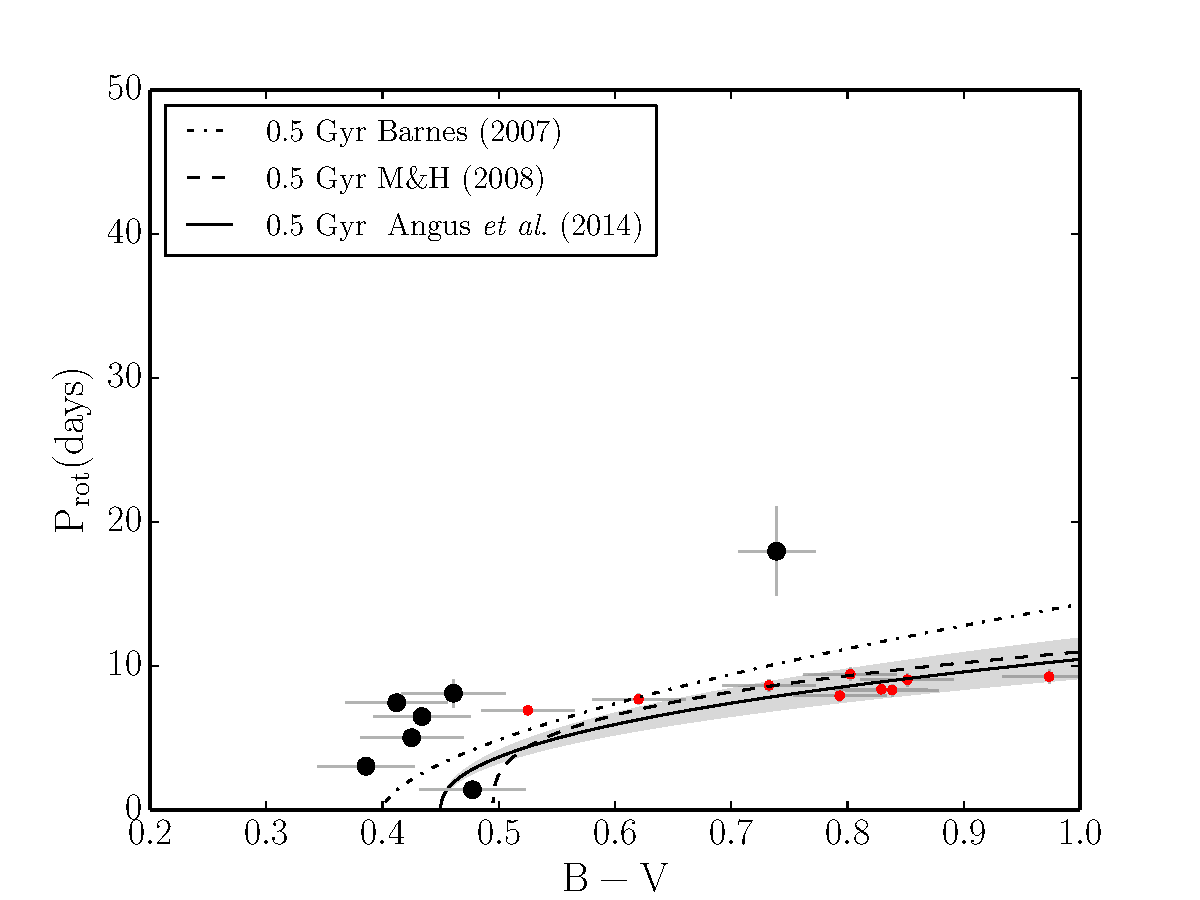
\includegraphics[width=2in, clip=true, trim=0 0 0.5in 0]{/Users/angusr/Python/Gyro/plots/p_vs_bv0.png}
        }
	\subfigure[1 Gyr (age of NGC 6811)]{
            \label{fig:1gyr}
	    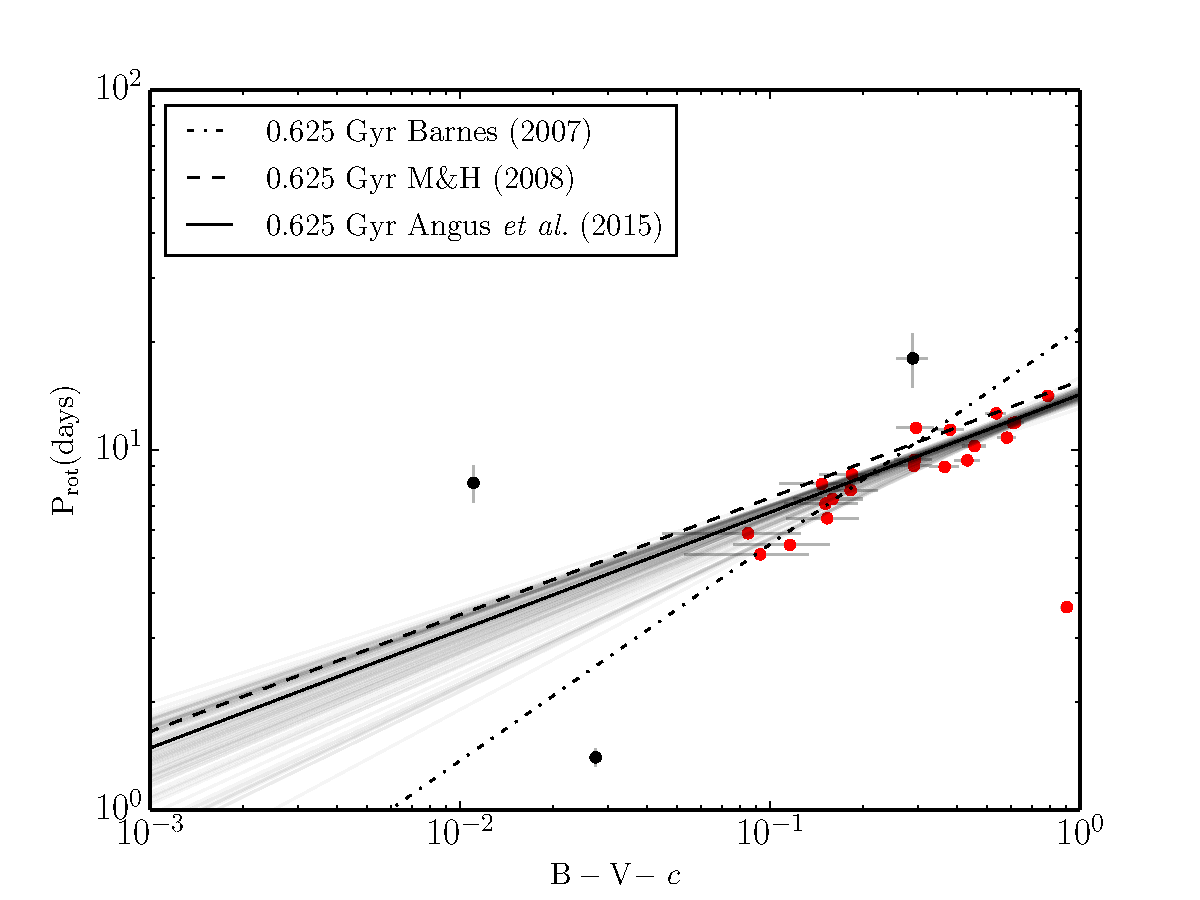
\includegraphics[width=2in, clip=true, trim=0 0 0.5in 0]{/Users/angusr/Python/Gyro/plots/p_vs_bv1.png}
        }
	\subfigure[2 Gyr]{
            \label{fig:2gyr}
	    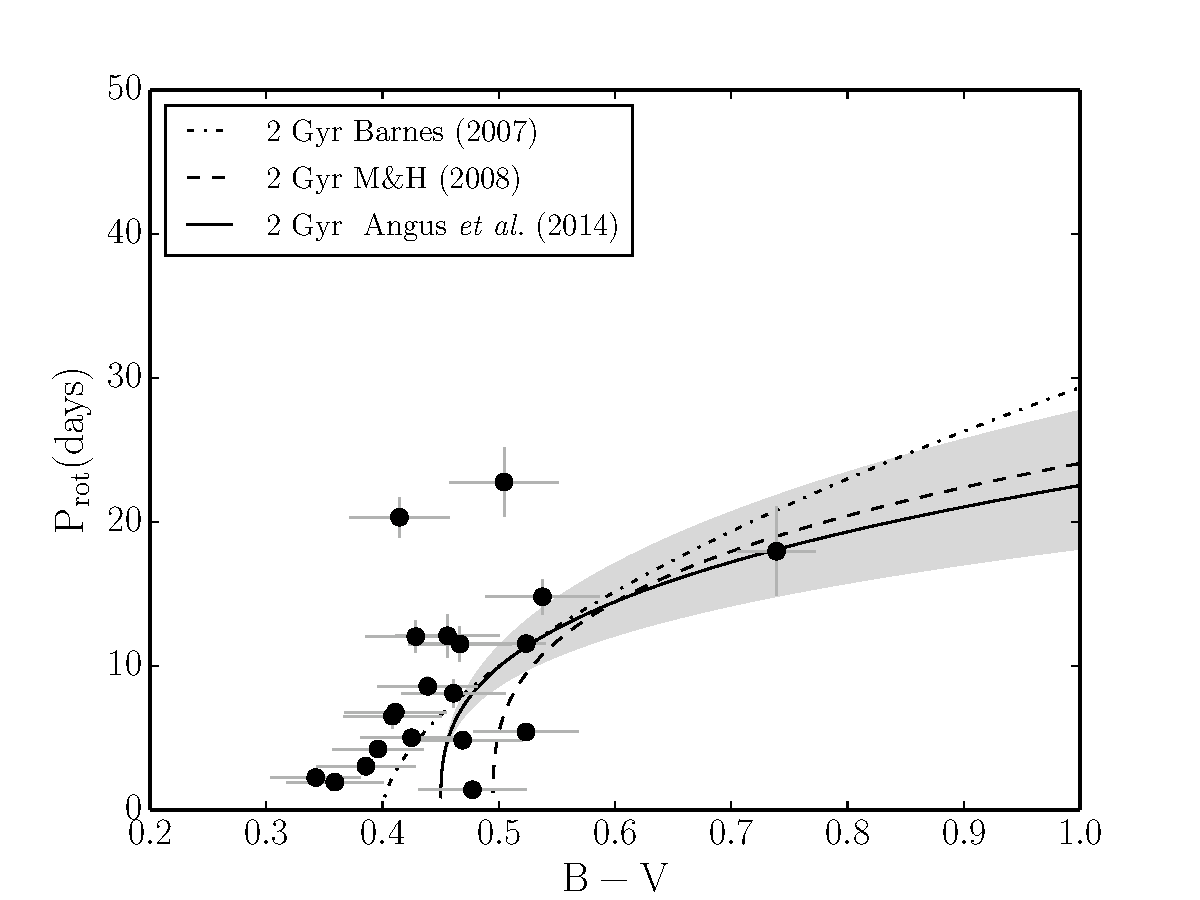
\includegraphics[width=2in, clip=true, trim=0 0 0.5in 0]{/Users/angusr/Python/Gyro/plots/p_vs_bv2.png}
        }
	\subfigure[3 Gyr]{
            \label{fig:3gyr}
	    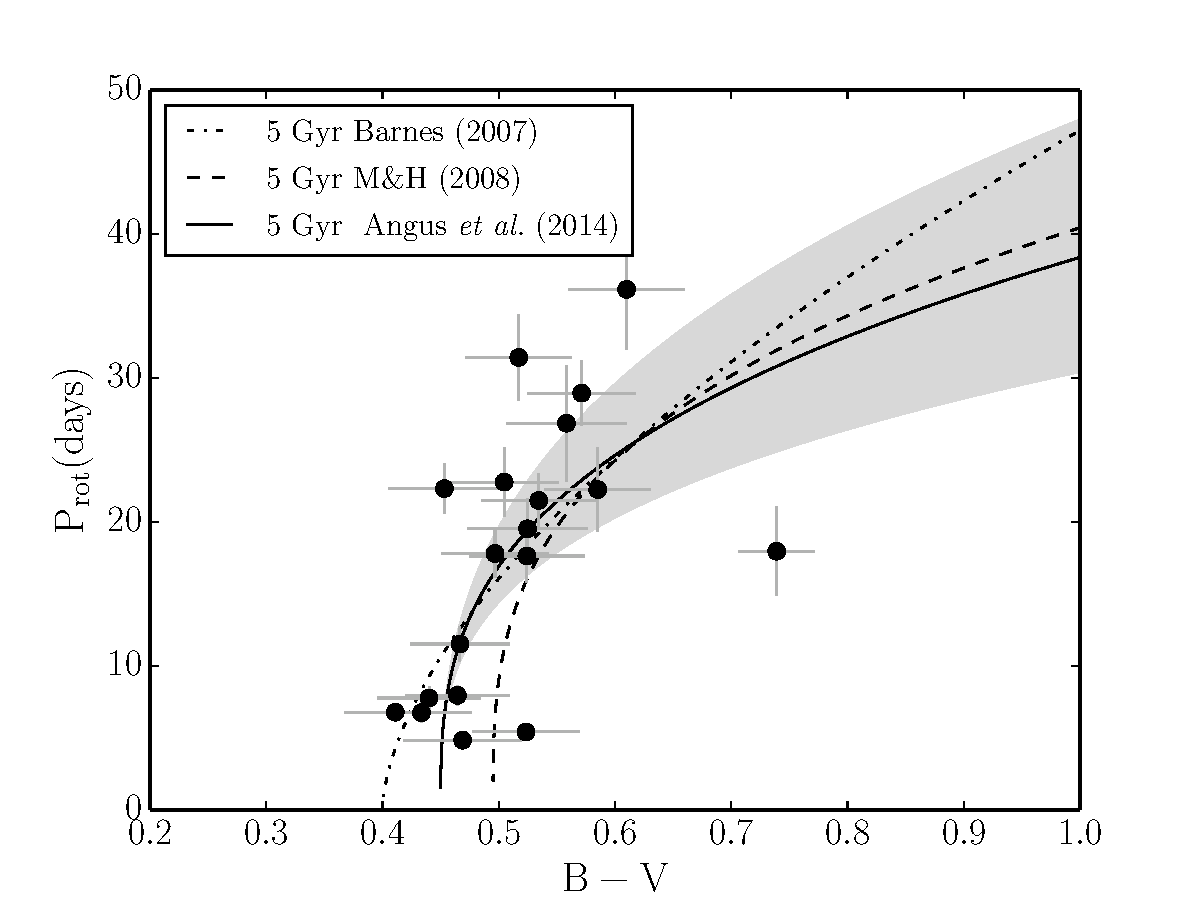
\includegraphics[width=2in, clip=true, trim=0 0 0.5in 0]{/Users/angusr/Python/Gyro/plots/p_vs_bv3.png}
        }
	\subfigure[4.568 Gyr (Solar age)]{
            \label{fig:sungyr}
	    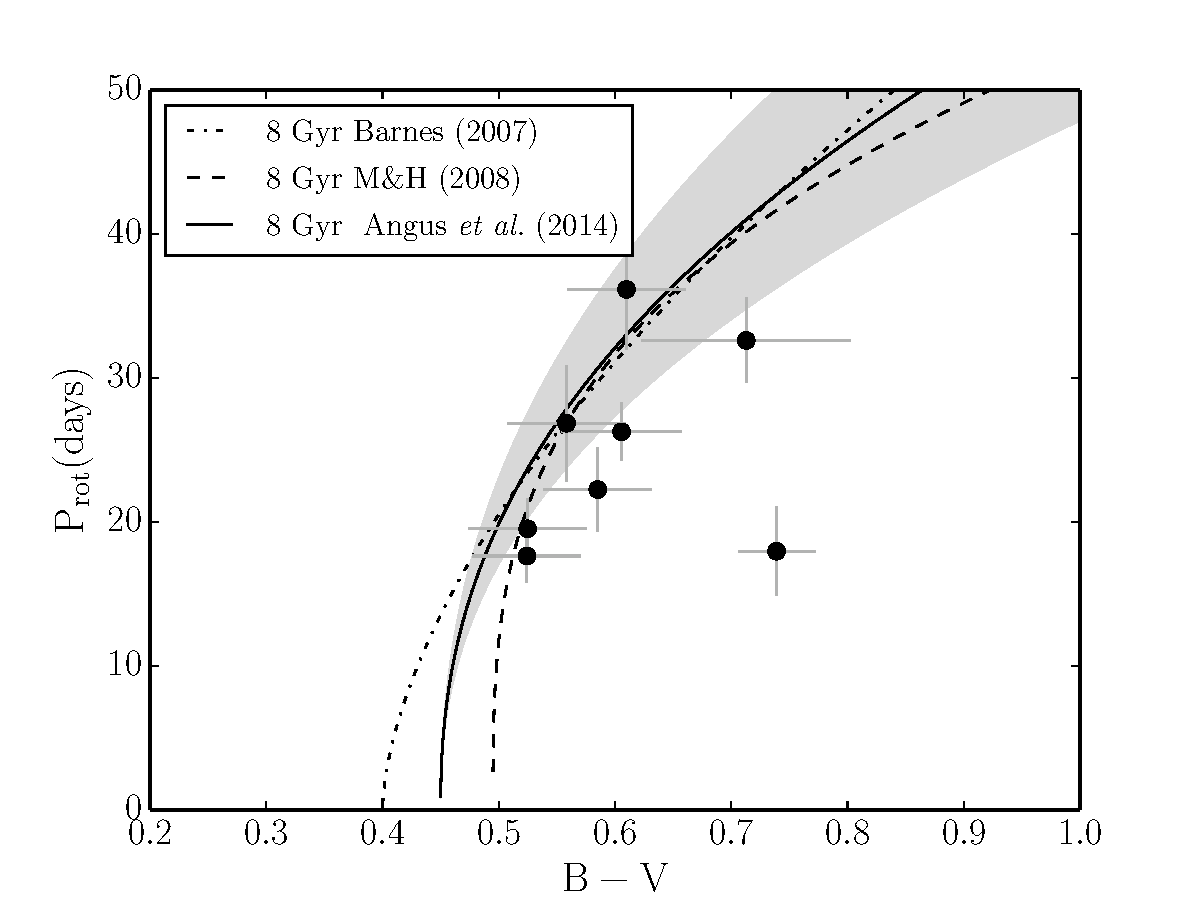
\includegraphics[width=2in, clip=true, trim=0 0 0.5in 0]{/Users/angusr/Python/Gyro/plots/p_vs_bv4.png}
        }
	\subfigure[6 Gyr]{
            \label{fig:6gyr}
	    \includegraphics[width=2in, clip=true, trim=0 0 0.5in 0]{/Users/angusr/Python/Gyro/plots/p_vs_bv5.png}
        }
	\subfigure[8 Gyr]{
            \label{fig:8gyr}
	    \includegraphics[width=2in, clip=true, trim=0 0 0.5in 0]{/Users/angusr/Python/Gyro/plots/p_vs_bv6.png}
        }
	\subfigure[10 Gyr]{
            \label{fig:13gyr}
	    \includegraphics[width=2in, clip=true, trim=0 0 0.5in 0]{/Users/angusr/Python/Gyro/plots/p_vs_bv7.png}
        }
    \end{center}
    \caption{ \prot vs B-V colour for dwarfs within 1$\sigma$ of the reference age with the new gyrochronology relation and \citet{Barnes2007}, and \citet{Mamajek2008} for comparison. Asteroseismic targets are circles and cluster and field stars are red triangles. The shaded region represents the 16th and 84th percentile uncertainties.
     }
   \label{fig:subfigures2}
\end{figure}

\begin{figure}[ht]
\begin{center}
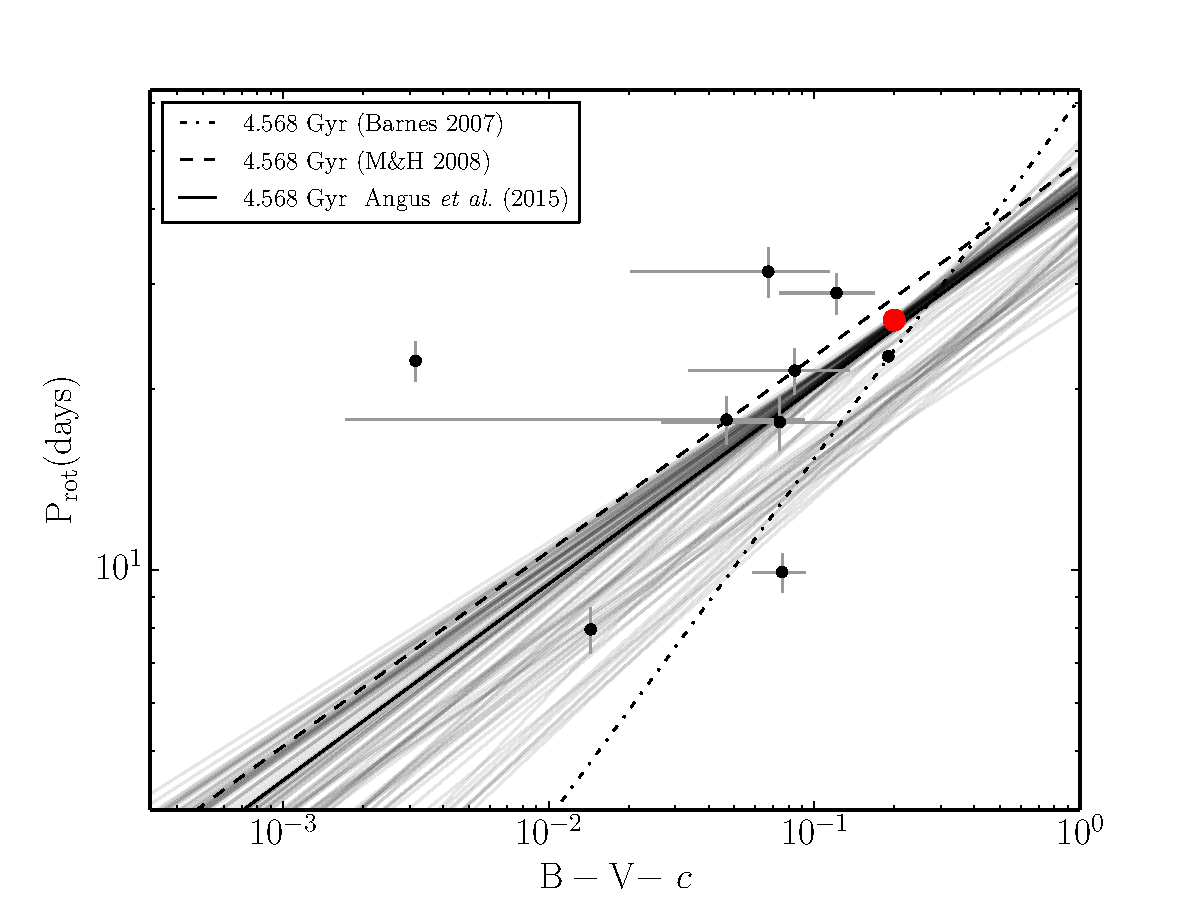
\includegraphics[width=6in, clip=true, trim=0 0 0.5in 0]{/Users/angusr/Python/Gyro/plots/p_vs_bv_solar.png}
\caption{Rotation period vs B-V colour for dwarfs with age within 1$\sigma$ of the Sun's age, 4.568 Gyr. The grey stars are hotter than 6250 K. The Sun is shown as a large grey circle.}
\label{fig:p_vs_bv_solar}
\end{center}
\end{figure}
%
\begin{figure}[ht]
\begin{center}
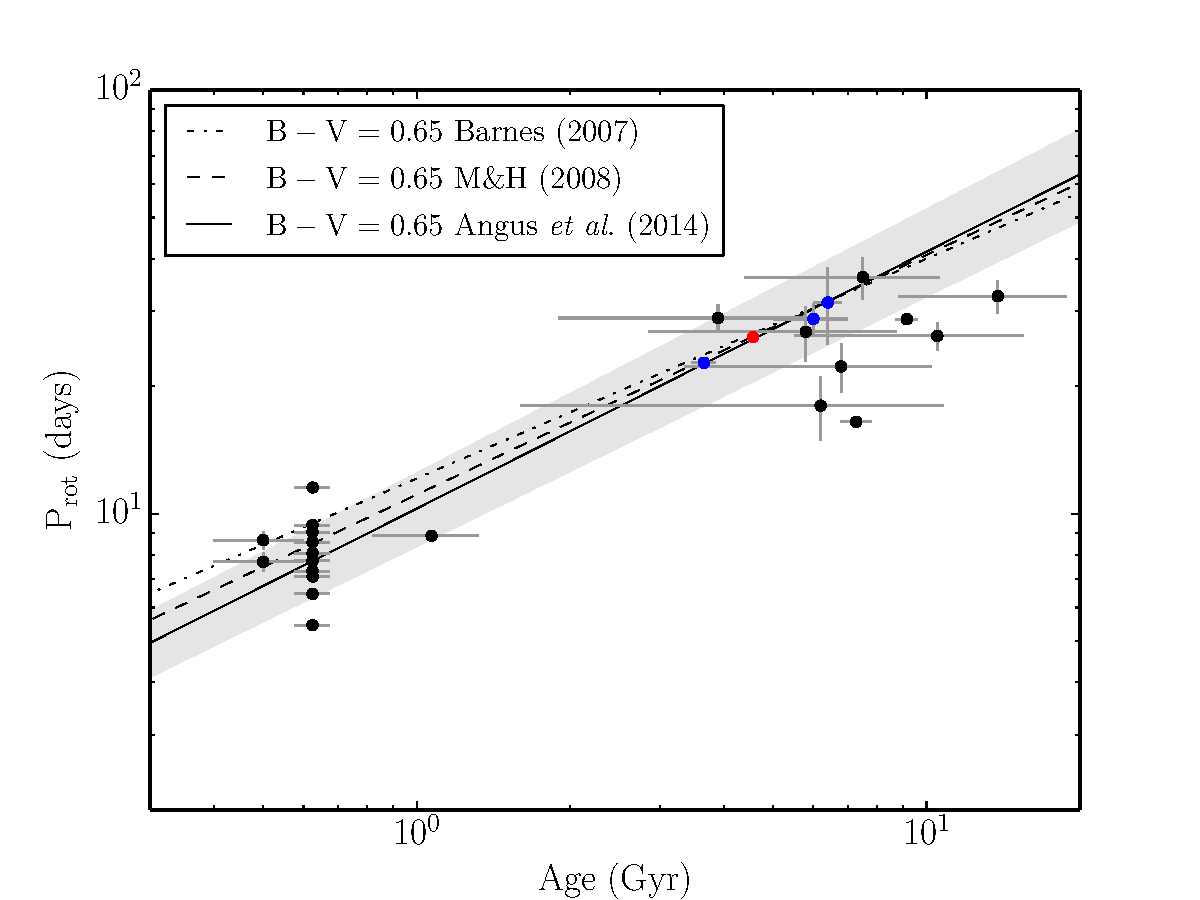
\includegraphics[width=6in, clip=true, trim=0 0 0.5in 0]{/Users/angusr/Python/Gyro/plots/p_vs_a_solar.png}
\caption{Rotation period vs age for cool dwarfs with colour within 10\% of the Sun's: 0.65, with gyrochronology relations of \citet{Barnes2007}, \citet{Mamajek2008} and this work. The shaded region represents the 16th and 84th percentile uncertainties. The Sun is shown as a large grey circle.}
\label{fig:p_vs_a_solar}
\end{center}
\end{figure}

There are a few potential explanations for the differences between previous and newly calibrated relations.
The first, and most obvious, is simply that the Sun is not a typical rotator for its age - it is slowly rotating.
Previous calibrations draw their age dependence almost exlusively from the Sun, assuming that it is representative of other stars with the same rotation period and mass.
In light of these new data, it may be time to reassess the `Sun is a representative star' viewpoint.
Another plausible explanation is that the asteroseismic ages are systematically too old; this would make the Sun appear to be slowly rotating for its age.
Alternatively, the ACF method could be underestimating rotation periods.
{\color{red} Do we have any reason to believe either of these to be true?}
% could test this

% NON-NARROW RELATIONSHIP

The goal of gyrochronology in general is to provide a means of predicting the age of a star, given observations of its \teff, or colour, and rotation period.
The `narrowness' of the gyrochronology relation has hitherto been an unknown; do the three properties, age, mass and rotation period truely lie on an infinitely narrow plane?
Does age depend solely on rotation period and mass, or do other variables influence stellar spin down---perhaps only becoming important after many Myrs?
Metallicity, for example, could play a role---a future study might explore the influence of this property on angular momentum loss rate.
Unfortunately, we cannot answer these questions here: the asteroseismic ages are noisy and observational and intrinsic scatter are ambiguously interwoven.
A future study might include an extra parameter that describes the `width' of the gyrochronological plane and attempt to detect an element of scatter above the noise level.
The success of this approach would strongly depend on having truely representative observational uncertainties.

% THEORY

A rift exists between theory and observation in the field of gyrochronology.
Attempts to unite the two are ongoing \citep{Barnes2011}, \citep{vanSaders2013}.
The gyrochronology relation of \citet{Barnes2010} attemps to reconcile empirical gyrochronology with physical models.
However it requires knowledge of stars' initial rotation periods---in practise, this information is rarely (if ever) available.

% Core-envelope decoupling

{\color{red} to do: read up on sample biases.}
Asteroseismic surveys are biased towards relatively quiet, bright stars, slightly more massive than the Sun.
There are very few young K stars in the \citet{Chaplin2013} sample---presumably because these stars are active.
Unfortunately, those stars that are ideal asteroseismic targets are often less-than-ideal for a rotation survey.

% List of figures:
% marginalised plot
% completeness plot?

\section{Conclusions}
\label{sec:conclusions}

We have calibrated the relation between rotational period, B-V colour and age for MS stars with \teff $<$ 6250 K using 153 Kepler asteroseismic targets, as well as 5 field stars and 260 cluster stars with precise age measurements.
We find that the Sun is no longer well described by gyrochronology---it appears to be slowly rotating for its age and mass compared with the asteroseismic stars.
However it is possible that systematic overestimation of the asteroseismic star's ages, or underestimation of their rotation periods is responsible for this discrepancy (note that the field stars are consistent with the Sun).
This will become clear when more stars in the asteroseismic sample have precise age measurements from individual oscillation mode analysis.
These precise ages will continue to be published over the coming months and years.
Once those stars for which it is possible to measure precise ages (the $\sim$ 150 in the \citet{Chaplin2013} sample with high signal-to-noise), this gyrochronology relation will be updated.

The future looks bright for gyrochronology; K2 will provide rotation periods for hundreds of stars lying in old clusters, with precisely known ages.
These data will be invaluable for gyrochronology and will provide a far more comprehensive view of the period-mass-age plane than has been possible so far.
The TESS spacecraft will also deliver high precision photometry, suitable for both asteroseismic studies and rotation period measurement.
We are entering an era where cluster studies and asteroseismology will deliver precise ages for stars with measureable rotation periods: the picture of gyrochronology will continue to advance over the coming years.

The code used in this project can be found at https://github.com/RuthAngus/Gyro.
We would like to thank Eric Mamajek, Marc Pinsonneault, Sydney Barnes, Steve Kawaler, Jerome Bouvier, Daniel Mortlock and David Hogg for useful insight and discussion.

% \section{Appendix}
%
% \subsection{Probability theory}
%
% For the low-mass MS stars the joint probability can be factorised as:
%
% \begin{equation}
%   p(\hat{A}_n,\hat{P}_n,\hat{C}_n,A_n,P_n,C_n,G_n|\theta) =
%   p(A_n,P_n,C_n,G_n|\theta) p(\hat{A}_n|A_n)
%   p(\hat{P}_n|P_n) p(\hat{C}_n|C_n) p(\hat{G}_n|G_n),
% \label{eq:jointprob}
% \end{equation}
%
% \begin{equation}
% 	\propto p(A_n|P_n,C_n,G_n,\theta) p(\hat{A}_n|A_n)
% 	p(\hat{P}_n|P_n)p(P_n) p(\hat{C}_n|C_n)p(C_n) p(\hat{G}_n|G_n)p(G_n) dA_n dP_n dC_n dG_n
% \label{eq:jointprob}
% \end{equation}
%
% and the marginalised likelihood for a single star can be written as the sum of the individual star likelihoods over the three different regimes, k:
%
% \begin{multline}
% p(\hat{P}_n,\hat{A}_n,\hat{C}_n,\hat{G}_n|\theta,C_K)  = \\
% \sum_{k=1}^3\int p(A_n,C_n,P_n,G_n|\theta,C_K)
% p(\hat{A}_n|A_n) p(\hat{C}_n|C_n) p(\hat{P}_n|P_n) p(\hat{G}_n|G_n)
% {\rm d}A_n {\rm d}C_n {\rm d}P_n {\rm d}G_n,
% \end{multline}
% \label{eq:L1}
%
% where $p(A_n,C_n,P_n,G_n|\theta,C_K)$ is different in the three regimes, as listed in table \ref{tab:jprob}.
%
% \begin{deluxetable}{lc}
% \label{tab:jprob}
% \tablewidth{0pc}
% \tablecaption{Probability of hidden variables for the three populations.}
% \tablehead{
% \colhead{Regime}&
% \colhead{Joint probability distribution}}
% \startdata
% Low mass, MS & $p(A_n,P_n,C_n,G_n|\theta) = p(C_n|C_K) p(G_n) p(P_n) p(A_n|C_n,P_n,\theta)$ \\
% High mass, MS & $p(A_n,P_n,C_n,G_n|Y, V) = p(P_n) p(C_n) p(G_n) p(A_n|Y, V)$  \\
% Subgiants & $p(A_n,P_n,C_n,G_n|Z, U) = p(C_n) p(G_n) p(P_n) p(A_n|Z, U)$ \\
% \enddata
% \end{deluxetable}

\bibliographystyle{plainnat}
\bibliography{Gyro_paper}

\begin{figure}[ht]
\begin{center}
\includegraphics[width=6in, clip=true, trim=0 0 0.5in 0]{/Users/angusr/angusr/ACF/ACF2/PDCQ3_output/plots_acf/3223000_full.png}
\caption{\emph{Top:} Quarter 3 PDC-MAP light curve of KIC 3223000. \emph{Middle:} The light curve with linear trends removed and gaps interpolated across. \emph{bottom:} The ACF. This star shows high amplitude variability. We measured a rotation period of 4.86 $\pm$ 0.05 days}
\label{fig:lc}
\end{center}
\end{figure}
%
\begin{figure}[ht]
\begin{center}
\includegraphics[width=6in, clip=true, trim=0 0 0.5in 0]{/Users/angusr/angusr/ACF/ACF2/PDCQ3_output/plots_acf/3429205_full.png}
\caption{\emph{Top:} Quarter 3 PDC-MAP light curve of KIC 3429205. \emph{Middle:} The light curve with linear trends removed and gaps interpolated across. \emph{bottom:} The ACF. This star does not display high amplitude variability---no rotation period was measured for this target.}
\label{fig:lc}
\end{center}
\end{figure}
%
\begin{figure}[ht]
\begin{center}
\includegraphics[width=6in, clip=true, trim=0 0 0.5in 0]{/Users/angusr/angusr/ACF/ind_qs_figs/3223000.pdf}
\caption{Period measurements for quarters 3 - 16 of star `KIC 7771282'. The blue solid line indicates the median value and the shaded blue region marks its 15\% margin. The blue dashed line with surrounding shaded area indicates one half of the median period measurement with 15\% margin.  More than two thirds of the period measurements were present and consistent to within 15\% of the median for this star, so it passed the selection process.}
\label{fig:ind_qs}
\end{center}
\end{figure}

\end{document}
